\documentclass[conference]{IEEEtran}
%\IEEEoverridecommandlockouts
% The preceding line is only needed to identify funding in the first footnote. If that is unneeded, please comment it out.
%\usepackage{cite}
\usepackage{amsmath,amssymb,amsfonts}
\usepackage{algorithmic}
\usepackage{graphicx}
\usepackage{textcomp}
\def\BibTeX{{\rm B\kern-.05em{\sc i\kern-.025em b}\kern-.08em
    T\kern-.1667em\lower.7ex\hbox{E}\kern-.125emX}}
\usepackage{mathtools}

%\usepackage[backend=biber]{biblatex}
%\addbibresource{references.bib}

\DeclareMathOperator*{\argmin}{argmin}
\DeclareMathOperator{\E}{\mathbb{E}}
\newcommand{\norm}[1]{\left\lVert#1\right\rVert}

\renewcommand*{\bibfont}{\footnotesize}
\renewcommand\IEEEkeywordsname{Index Terms}
\IEEEoverridecommandlockouts

\begin{document}

\title{Optimal Energy Management of Electric Vehicles with Dual Storage}

\author{Alok~Deshpande,~\IEEEmembership{Student Member,~IEEE}, and~Joshua~A.~Taylor,~\IEEEmembership{Member,~IEEE}%
\thanks{A. Deshpande and J.A. Taylor are with The Edward S. Rogers Sr. Department of Electrical \& Computer Engineering, University of Toronto, Toronto, Ontario, Canada, M5S 3G4. Email: \{\texttt{alok.deshpande@mail.,josh.taylor@}\}\texttt{utoronto.ca}}%%
% \thanks{Manuscript received X; revised X.}
}

\maketitle

\begin{abstract}
Combining storages with different characteristics can improve the performance and lifetime of electric vehicles. For example, a supercapacitor and a battery together can handle large power transfers from acceleration and regenerative braking while protecting the battery from degradation. In this paper, we use approximate dynamic programming to design a policy for power sharing between dual storage devices. We write the dynamic program as a linear program and use basis functions to approximate the optimal value function. Numerical results show that this suboptimal policy can approximate the optimal policy with low error given a sufficient number of basis functions.
%This document is a model and instructions for \LaTeX.
%This and the IEEEtran.cls file define the components of your paper [title, text, heads, etc.]. *CRITICAL: Do Not Use Symbols, Special Characters, Footnotes, 
%or Math in Paper Title or Abstract.
\end{abstract}
\begin{IEEEkeywords}
Electric vehicles, approximate dynamic programming, batteries, supercapacitors.\end{IEEEkeywords}

\section{Introduction}
Battery life is an important consideration in electric vehicle (EV) operation. An aging battery experiences a drop in energy capacity \cite{8449100}, which reduces the maximum distance that can be travelled on a single charge. One promising way to prolong battery life is to use a hybrid energy storage system, composed of a combination of a battery and a secondary energy storage in parallel \cite{thounthong2009energy}, such as a supercapacitor \cite{thounthong2009energy,bambang2014energy,7939849}. 

Dynamic programming (DP) has previously been been applied in this context to determine an optimal sequence of controls --- that is to say, energy discharges from the battery and supercapacitor --- which satisfies a sequence of energy demands. Reference \cite{su2013modeling} has applied DP to a single battery. We extend this to the two-storage case. References \cite{8330176} and \cite{8315074} have both solved the problem under the assumption of an infinite horizon, and we do so similarly.

Our approach differs from these papers as follows. We first reformulate the infinite horizon DP as a linear program (see, e.g., \cite{Bertsekas:2007:DPO:1396348}). We then construct an approximation using the basis function technique given in \cite{deFarias:2003:LPA:970869.970918}, and generate basis functions for the approximation using the methods of \cite{Bellman:1957} and \cite{Bellman1962}. %\cite[pp. 323--324]{Bellman1962}.

We physically model the problem in Section II and pose the infinite horizon DP in Section III. In Section IV, we describe the basis functions we use to approximate the value function. Finally, in Section V, we show numerical results for a vehicle with a battery and a supercapacitor. 


\section{Model}
In this section, we model the two storage device optimization problem. Let $E_{h}(t)$ and $D_{h}(t)$ denote the energy stored in and energy discharged from device $h$ at time instant $t$, respectively. Here $h=1$ refers to the battery and $h=2$ refers to the supercapacitor. Let $L(t)$ be the energy demand imposed on the system, and $C_{h}(t)$ be the energy moved into device $h$ by charging at time $t$. We define the state to be $x(t)=[E_{1}(t),E_{2}(t),L(t)]^{T}$ and the control to be $u(t)=[D_{1}(t),D_{2}(t)]^{T}$. Note that $C_{2}(t)$ is not part of the control because it is a dependent variable through the energy supply-demand balance, as explained below.

The state equation for the battery without regenerative braking is:
\begin{equation} \label{eq:BattStateEqn}
    E_{1}(t+1)=\beta_{1}E_{1}(t)-\frac{1}{\alpha_{1}^{D}}D_{1}(t)
\end{equation} Likewise, the state equation for the supercapacitor is:
\begin{equation} \label{eq:SupercStateEqn}
    E_{2}(t+1)=\beta_{2}E_{2}(t)+\alpha_{2}^{C}C_{2}(t)-\frac{1}{\alpha_{2}^{D}}D_{2}(t)
\end{equation} Here, $\alpha^{C}_{h}$ and $\alpha^{D}_{h}$ respectively denote the charging and discharging efficiencies of device $h$, and $\beta_{h}$ is the leakage of device $h$. The energy supply-demand balance also imposes the following constraint: $D_{1}(t) + D_{2}(t) - C_{2}(t) = L(t)$. We write the state transition more concisely as $x(t+1)=f(x(t),u(t),w(t))$, where $w(t)$ is a bounded random variable described below.

In this model, the energy in storage device $h$ is bounded in the range $E_{h}^{\min}\leq E_{h}(t)\leq E_{h}^{\max}$ where $E_{h}^{\max}$ is the upper bound and $E_{h}^{\min}$ is the lower bound, normally equal to zero. We discretize this range into $N_{h}$ energy levels for the device $h$, and define $N=N_{1}N_{2}$. The charging and discharging energies are constrained to the ranges $0\leq C_{h}(t)\leq C_{h}^{\max}$ and $0\leq D_{h}(t)\leq D_{h}^{\max}$, where $C_{h}^{\max}$ and $D_{h}^{\max}$ are the upper bounds on the charging and discharging rates, respectively. They are also discretized, as explained below after \eqref{eq:initCostFnc}.


There are two relevant costs in this model. The first is the loss of energy due to transfers between the devices, which is:
\begin{displaymath}
\bigg(\frac{1}{\alpha_{1}^{D}}-1\bigg)D_{1}(t)+(1-\alpha_{2}^{C})C_{2}(t)+\bigg(\frac{1}{\alpha_{2}^{D}}-1\bigg)D_{2}(t)
\end{displaymath} The other cost is that for the discharge rate for the battery, simply given by $K(D_{1}(t))^{2}$. Here $K$ is a weighting for this cost relative to the cost of energy loss. This cost penalizes larger power transfers \cite{bambang2014energy}, which cause greater battery degradation. We define the stage cost of the optimization problem to be:
\begin{align*}
    g(x(t),u(t),w(t))=&\bigg(\frac{1}{\alpha_{1}^{D}}-1\bigg)D_{1}(t) +(1-\alpha_{2}^{C})C_{2}(t)\\& +\bigg(\frac{1}{\alpha_{2}^{D}}-1\bigg)D_{2}(t) +K(D_{1}(t))^{2}
\end{align*}

We collect this objective and the above constraints in the below convex optimization problem:
\begin{multline} \label{eq:initCostFnc}
    \min \mathop{\E}\Biggl[\sum_{t=0}^{T-1}g(E_{1}(t),E_{2}(t),L(t),D_{1}(t),D_{2}(t))\Biggr]
\end{multline}
subject to
\begin{flalign*}
& E_{h}^{\min}\leq E_{h}(t)\leq E_{h}^{\max}, h=1,2\\
& 0\leq C_{2}(t)\leq C_{2}^{\max}\\
& 0\leq D_{h}(t)\leq D_{h}^{\max}, h=1,2\\
& D_{1}(t) + D_{2}(t) - C_{2}(t) = L(t)\\
& E_{1}(t+1)=\beta_{1}E_{1}(t)-\frac{1}{\alpha_{1}^{D}}D_{1}(t)\\
& E_{2}(t+1)=\beta_{2}E_{2}(t)+\alpha_{2}^{C}C_{2}(t)-\frac{1}{\alpha_{2}^{D}}D_{2}(t)
\end{flalign*}
Note that the energy balance equality constraint can be substituted into the objective and the charging inequality constraints, which reduces the decision vector to $u=[D_{1},D_{2}]^{T}$. The range of the discharged energies for each device $h$, $0\leq D_{h}(t)\leq D_{h}^{\max}$, is discretized into $\rho_{h}$ levels, which means that the number of possible solutions, $u(t)$, at each stage of the DP is $\rho=\rho_{1}\rho_{2}$.

The optimal value function \eqref{eq:initCostFnc} may be expressed in the general form:
\begin{equation} \label{eq:FHDP}
	J_{0}(x(0))=\min \mathop{\E}_{w}\left[\sum_{t=0}^{T-1}g(x(t),u(t),w(t))\right]\end{equation}
The optimization \eqref{eq:FHDP} may then be written as the DP:
\begin{displaymath}
J_{t}(x(t))=\min_{u(t)} g(x(t),u(t)) + \mathop{\E}_{w(t)}\left[J_{t+1}(f(x(t),u(t),w(t)))\right]
\end{displaymath}
starting from $J_{T}(x(T))=0$. This is subject to the same constraints as \eqref{eq:initCostFnc}, which can be expressed as the set:
\begin{flalign*}
    \Omega = \Biggl\{& (E_{1},E_{2},L,D_{1},D_{2})\mid 
                E_{h}^{\min}\leq E_{h}\leq E_{h}^{\max}, h=1,2\\
                & 0\leq C_{2}(t)\leq C_{2}^{\max}\\
                & 0\leq D_{h}(t)\leq D_{h}^{\max}, h=1,2\\
                & E_{1}(t+1)=\beta_{1}E_{1}(t)-\frac{1}{\alpha_{1}^{D}}D_{1}(t)\\
                & E_{2}(t+1)=\beta_{2}E_{2}(t)+\left(\alpha_{2}^{C}C_{2}(t)-\frac{1}{\alpha_{2}^{D}}D_{2}(t)\right)\Biggr\}
\end{flalign*} where $C_{2}=D_{1}(t)+D_{2}(t)-L(t)$, using the energy balance constraint.

In this model, $L(t)$ is a random quantity which is observed at time $t$ before the control $u(t)$ is applied because the controller must have full knowledge of the demand. It evolves according to $L(t+1)=w(t)$. Note that $w(t)$ depends on the energy in the subsequent state, $E_{1}(t+1)$ and $E_{2}(t+1)$. This is because the demand at any iteration cannot exceed the total current energy at that iteration. Based on this requirement, the random demand is bounded to the range $0\leq L \leq L^{\max}=E_{1}^{\max}+E_{2}^{\max}$. It is also discretized into $M=N_{1}+N_{2}$ levels in accordance with the discretization of $E_{h}$.

Let $X$ be the set of values the discretized state, $x(t)$, can take. As the state evolves with each iteration of the DP, the subsequent state, $x(t+1)=f(x(t),u(t),w(t))$, may not lie in $X$. We use interpolation to determine the value function at the state $x(t+1)\not\in X$. First, we define three sets: $W$ as the set of random demands, indexed by $k\in\{1,...,M\}$; Y as the set of points $[E_{1},E_{2}]^{T}$, indexed by $\gamma \in\{1,...,N\}$; and $U$ as the set of controls, indexed by $p\in\{1,...,\rho\}$. By the above definition, $X=Y\times W$. We index $X$ by $i\in\{1,...,NM\}$. We use subscripts to index the elements each set, e.g., $x_{i}$ is the $i^{th}$ element in set $X$.

We note that no interpolation is needed for the demand, $L(t)$, because it is drawn from a discrete distribution. Hence, we use bilinear interpolation for the weightings, as described in \cite[p.~319]{MultiLinInterp} and elsewhere. To  compute the optimal policy, we can encode the interpolation scheme in a constant matrix $F_{p}$ for each control $u_{p}$. This is to say that if we let $x_{i}$ be any state in $X$ and $x_{j}=f(x_{i},u_{p},w_{k})$ be the state at time $t+1$, the entry $(i,j)$ of $F_{p}$ contains the weight of $J_{t+1}(x_{i})$ that contributes to $J_{t+1}(x_{j})$.

We express our model as a Markov chain to enable a linear programming formulation. Let $p_{i,j}(u_{p})=P(x_{j}| x_{i},u_{p})$ be the probability of moving from $x_{i}\in X$ to $x_{j}$ by applying control $u_{p}\in U$. For $p_{i,j}(u_{p})$ to be non-zero, the next state $x_{j}$ must be accessible from the current state, i.e., $x_{j}=f(x_{i},u_{p},w_{k})$. The only random variable in $f(x_{i},u_{p},w_{k})$ is $w_{k}\in W$, so we may express this instead as a probability of $w_{k}$, which is $P(w_{k} | x_{i},u_{p})$. The transition probability is then:
\begin{equation} \label{eq:TransMtx}
p_{i,j}(u_{p})=
\left\{
\begin{array}{l}
P(w_{k}|x_{i},u_{p}) \hspace{0.3cm} \text{if} \hspace{0.2cm} x_{j}=f(x_{i},u_{p},w_{k})\\
0 \hspace{2.0cm} \text{otherwise}
\end{array}
\right.
\end{equation} We express this as a transition probability matrix $P_{p}$, whose entries are $p_{i,j}(u_{p})$ for control $u_{p}$.
%in the $p^{th}$ subset of rows 




\section{Infinite Horizon Approximation}
%\subsection{Infinite Horizon DP}
The length of each time period is very small relative to the total driving time. For example, each period might represent a second. If the total driving time is an hour, this means 3600 periods. This motivates the use of an infinite horizon approximation.

The infinite horizon DP is:
\begin{equation} \label{eq:DP}
J(x)=\min_{u} g(x,u) + \alpha\mathop{\E}_{w} \{J(f(x,u,w))\}
\end{equation} subject to $(x,u)\in\Omega$. Here $\alpha$ is a real-valued discount factor such that $0<\alpha<1$. Using this approximation, in the following sections we formulate an LP equivalent to this DP and use its solution to obtain the optimal policy. As a reminder, in the context of the hybrid storage problem, $x=(E_{1},E_{2},L)$ and $u=(D_{1},D_{2})$.


\subsection{Linear Programming Formulation}
We use an equivalent LP formulation of \eqref{eq:DP}. Let $\lambda\in\mathbb{R}^{MN}$ be a vector of the value function at each value in $X$, and let $g$ be a vector of the stage cost for each state-control pair. Then, the problem can be expressed as:
\begin{equation} \label{eq:LPfinal}
    \max_{\lambda} 1^{T} \lambda
    \hspace{1em}s.t.\hspace{1em}
    (\iota-\alpha \overline{P})\lambda \leq g
\end{equation} Here, $\iota=[I,...,I]^{T}$ is a matrix consisting of $\rho$ copies of the identity matrix and $\overline{P}=[(P_{1}F_{1})^{T},...,(P_{\rho}F_{\rho})^{T}]^{T}$ is a matrix consisting of matrices $P_{p}F_{p}$, structured as defined. %$P=diag(P_{1},...,P_{\rho})$ is a block diagonal matrix containing all the matrices $P_{p}$ along its diagonal
%Here, $\Lambda = [\lambda,\hdots, \boldsymbol{\lambda_{p}}]^{T}$ is a vector containing $\rho$ copies of vectors $\boldsymbol{\lambda_{p}}$. Each vector $\boldsymbol{\lambda_{p}}$ contains the current state values, $\lambda(x_{i})$, as its components.
%Likewise, the vector $F\boldsymbol{\lambda}$ contains P repeated vectors each containing the costs for next states $x_{j}$. And finally,
This is the final form of the LP exactly equivalent to the DP. 

\subsection{Optimal Policy}
The optimal policy my be constructed directly from the solution of the LP in \eqref{eq:LPfinal} \cite{Bertsekas:2007:DPO:1396348}. For $x\in X$ it is given by:

\begin{equation}
    u^{*}(x)=\argmin_{u} g(x,u)+\alpha \sum_{w} P(w|x,u)\lambda(f(x,u,w))
\end{equation}

We use bilinear interpolation to implement this policy for each state $x\not\in X$. %Let $x_{j}=f(x_{i}, u, w)$ be the next state, and let $u'(x_{j})$ be the interpolated suboptimal control to apply in this state. Specifically, define $x_{j}=(a_{j},b_{j},L_{0})$ where $L_{0}\in W$ is the demand in state $x_{i}$. Then, for the case where $x_{j}\not\in X$, we also approximate $u^{*}(x_{j})$ using bilinear interpolation as:

%\begin{equation}
%    u'(x_{j})=\sum_{l,m}q_{l,m,j}u^{*}(a_{l},b_{%m},L_{0})
%\end{equation} Here the state $(a_{l},b_{m},L_{0})\in X$ and $q_{l,m,j}$ is as defined above.


\section{Approximate Solution of LP}
Unfortunately, the state space is too large to use a fine discretization. To improve tractability, we approximate the value function with basis functions using the methodology of \cite{deFarias:2003:LPA:970869.970918}.

The approximate value function has the form $\Phi r$, where $\Phi \in \mathbb{R}^{MN\times R}$ is termed the design matrix and $r\in \mathbb{R}^R$ is a vector of weights. By choosing $R$ to be lower than $MN$, we reduce the size of the linear program. The $q^{th}$ column vector of $\Phi$ is a basis function denoted by $\phi_{q}$. In this section, we discuss methods to generate basis functions for the two-storage problem.

We give all basis functions equal weighting as no procedure exists for optimally determining the weights \cite{deFarias:2003:LPA:970869.970918, PatrascuReluEugen2004}. This leads to the following approximation, which is also an LP:
\begin{equation} \label{eq:ApproxLP}
    \max_{r} 1^{T} \Phi r
    \hspace{1em}s.t.\hspace{1em}
    (\iota-\alpha \overline{P})\Phi r \leq \boldsymbol{g}
\end{equation}

We use a combination of two types of basis functions: monomials, and vectors based on heuristic state aggregation. We describe these in the following two subsections.

\subsection{Monomials}
    We first use monomial basis functions \cite{bertsekas1995dynamic,478953}. Let $i$ be the index of state $x_{i}$. Then, the columns of $\Phi$ corresponding to monomials are of the form:
	
	\begin{displaymath}
        \Phi_{i,j}=x_{i}^{j-1}
    \end{displaymath} Here $i$ is the state index and $j$ is the column index. %, and $s(i)$ is a function which maps the state index to the associated state. %Again, a trade-off exists for increasing the value of $R$ between more decision variables and lower approximation error.

%\subsection{Random Vectors}
    %It is known that adding any linearly independent vector to an existing basis is guaranteed to decrease the approximation error. For that reason, we can sample randomly generated vectors until determining an additional vector that is linearly independent from the current basis, and subsequently add it to the basis. We can repeat this an arbitrary number of times to improve the approximation.


 \subsection{State Aggregation}
    
    %One may consider the case where multiple states have sufficiently similar optimal values that it is possible to approximate each optimal value by a single value for all the states in that aggregation.
    We use the heuristic of state aggregation to reduce the number of decision variables down to the number of aggregations of states \cite{5717627}. This is a less computationally expensive alternative to principal component analysis for this multidimensional problem, which is what \cite{PCA2015} and others apply to generate the basis functions for problems of lower dimension.%Specifically, each state in the aggregation has an associated index, so the basis functions are many-to-one functions of the state index $i$.
    
    Appropriate state aggregations depend on the problem, since the optimal value function varies. %By grouping state indices giving constant values of a function $b(i)$, we can determine the minimum number of aggregations to approximate the value function.
    However, each aggregation is defined to have approximate the same value of $\phi_{j}(x_{i})r_{j}$ for all states $x_{i}$ in that aggregation, where $j$ is the index of the aggregation. This implies that the matrix $\Phi$ must have the form:
    
    \begin{displaymath}
        \Phi_{i,j}=\left\{
            \begin{array}{l}
            1 \hspace{0.2cm} \text{if} \hspace{0.2cm} i\in H_{j}\\
            0 \hspace{0.2cm} \text{if} \hspace{0.2cm} i\not\in H_{j}
            \end{array}
            \right.
    \end{displaymath}where $H_{j}$ is the set $\{i|f_{j} = \phi_{j}(i)r_{j}\}=\{i|e_{j} = b(i)\}$. Here, $b(x_{i})$ is a model-specific function that is appropriately chosen to maximize the number of elements in $H_{j}$ for each $j$. $f_{j}$ and $e_{j}$ are, respectively, the approximate optimal value and the constant value of $b(x_{i})$ associated with the $j^{th}$ aggregation (basis function).
	
	Note that in order to determine one possible function $b(x_{i})$ for the given model, we run value iteration an arbitrary number of times to approximate $J^{*}_{j}(x_{i})$. This allows us to identify possible state aggregations.
    

\section{Numerical Examples}
We test our approach on an electric vehicle with a battery and a supercapacitor. In this paper, the optimization problems were solved numerically using Gurobi in CVX for varying sizes of state space, with all other variables kept constant. We used efficiency factors $\alpha^{C}_{1}=0.9$ and $\alpha^{D}_{1}=0.9$ for the battery, $\alpha^{C}_{2}=0.99$ and $\alpha^{D}_{1}=0.95$ for the supercapacitor, as well as a leakage factor of $\beta=0.99$ for both, based on the data in \cite{BattSupercapEff}. We also used a discount factor $\alpha=0.99$, weighting factor $K=2$, and $R'=10$ and $R=13$ for the number of basis functions. Starting from an initial energy state of $E_{1}=E_{1}^{\max}=10$ and $E_{2}=E_{2}^{\max}=5$, the problems were solved to determine the optimal policy offline. The random demand was constrained to $0\leq L \leq (E_{1}+E_{2})$, and the maximum discharge was limited to the total energy --- i.e. $D_{1}^{\max}=E_{1}^{\max}$ and $D_{2}^{\max}=E_{2}^{\max}$. Then, we applied demand sequences where the random load followed a uniform distribution for 10 periods to determine how the battery and supercapacitor behave under different conditions with the optimal policy.

The approximate LP was first solved offline. We then tested the optimal policy online for three cases of demand: constant demand, ramp demand (continuously increasing/decreasing), and fluctuating demand. Each demand sequence was randomly generated following a uniform distribution, for simplicity. %Importantly, no excess demands were permitted based on the state (total energy stored), such that the conditional probabilities could still change over time as the state evolved.

In the case of a constant or ramp demand, it was determined that the battery will tend to supply the majority of the energy. Figures \ref{fig:ConstDemand} and \ref{fig:RampDemand} illustrate these two cases for one set of initial conditions.
\begin{figure}[htbp]
\centerline{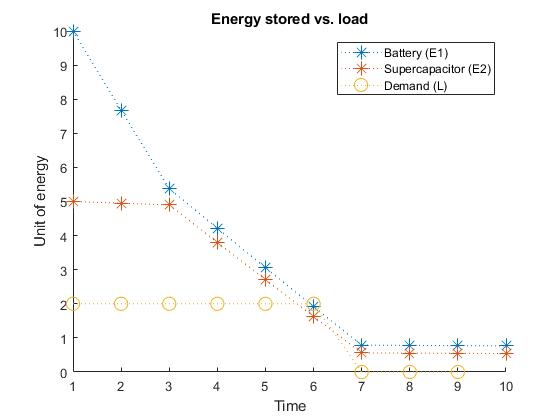
\includegraphics[scale=0.35]{EnergyStoredvsload_ConstantLoad(E1_max=10,E2_max=5).jpg}}
\caption{Testing optimal policy online with a constant demand sequence. Test size: $N_{1}=11$, $N_{2}=6$, $M=16$.}
\label{fig:ConstDemand}
\end{figure}
\begin{figure}[htbp]
\centerline{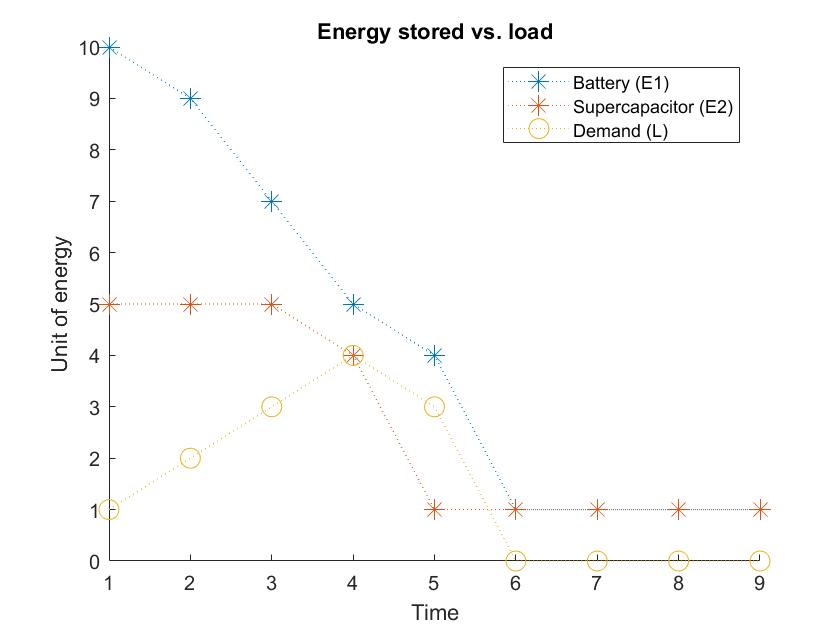
\includegraphics[scale=0.25]{EnergyStoredvsload_RampLoad(E1_max=10,E2_max=5).jpg}}
\caption{Testing optimal policy online with a ramp demand sequence. Test size: $N_{1}=11$, $N_{2}=6$, $M=16$.}
\label{fig:RampDemand}
\end{figure} This result is expected because there is relatively low cost for use of the battery under low demand or demand with limited fluctuation.

On the other hand, for highly fluctuating demand, the supercapacitor is used more, as illustrated in Figure \ref{fig:FluctuatingDemand}.
\begin{figure}[htbp]
\centerline{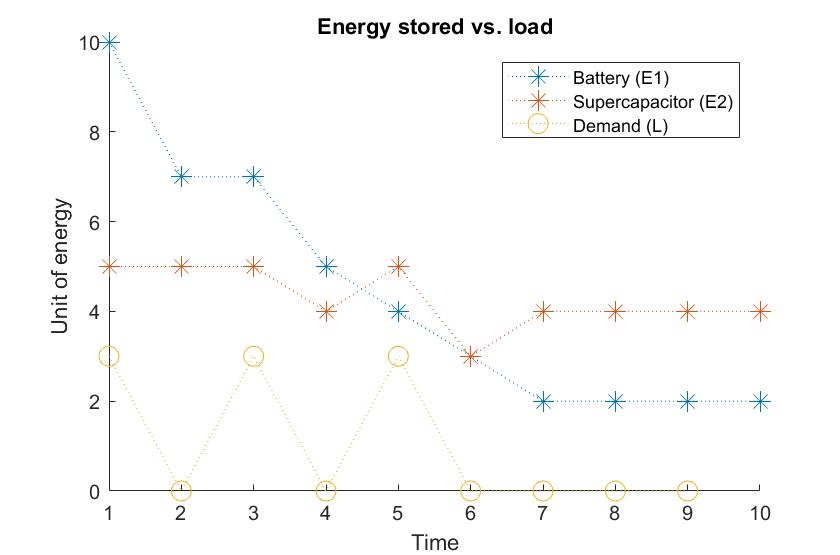
\includegraphics[scale=0.25]{EnergyStoredvsFluctuatingLoad(E1=10,E2=5).jpg}}
\caption{Testing optimal policy online with a fluctuating demand sequence. Test size: $N_{1}=11$, $N_{2}=6$, $M=16$.}
\label{fig:FluctuatingDemand}
\end{figure} Clearly, the supercapacitor is now discharged in the middle of the time sequence, at $t=6$. However, this is still not as much as expected. It was observed that by reducing the discharging efficiency of the battery, the supercapacitor is used more often (see Figure \ref{fig:FluctuatingDemand_LowBattEff}).
\begin{figure}[tbp]
\centerline{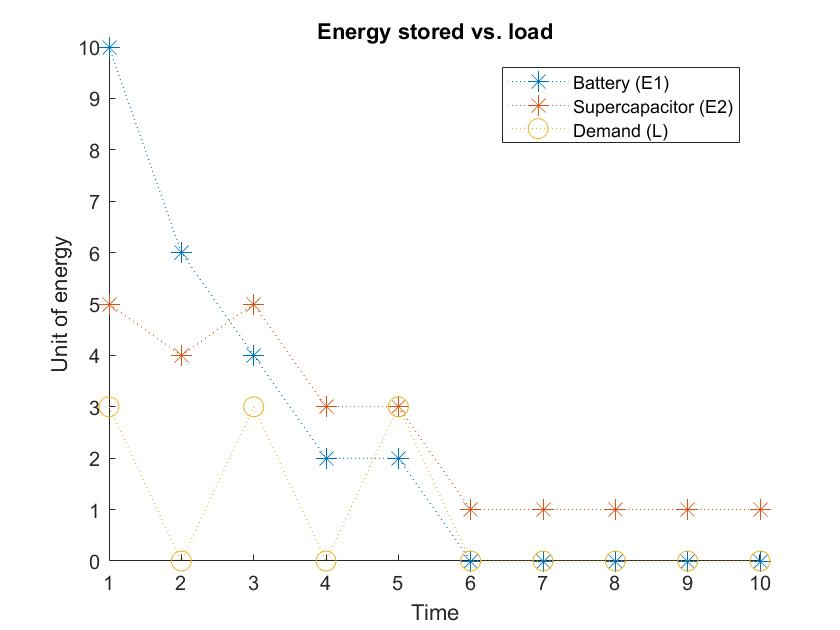
\includegraphics[scale=0.25]{EnergyStoredvsFluctuatingLoad_LowBattEff(E1=10,E2=5).jpg}}
\caption{Testing optimal policy online with a fluctuating demand sequence. Test size: $N_{1}=11$, $N_{2}=6$, $M=16$. Lower battery efficiency ($\alpha_{1}^{D}=50\%$).}
\label{fig:FluctuatingDemand_LowBattEff}
\end{figure} This shows that discharging the battery at the start of the sequence is still preferred because of the higher probability of large initial demands, unless the battery is inefficient.

One should also note how the battery is used to charge the supercapacitor, too. This can be seen, for example, in Figure 3 at time $t=4$, where there is no demand but there are still exchanges in the energy between the storage devices. This also confirms that the optimal policy is not myopic, since a trade-off is made between instantaneous transfer loss and satisfying fluctuating demands at a later time by preemptively charging the supercapacitor. Were it not for the benefits of the latter, there would be no reason for such energy exchanges.

Finally, in addition to testing the optimal policy, we also test the value function approximation. We quantify the approximation error for problems of small size. Figure \ref{fig:ApproxVsIter}, for example, illustrates the trade-off made between the approximation error and the number of iterations in solving the approximate LP, where the latter depends on the number of basis functions. \begin{figure}[tbp]
\centerline{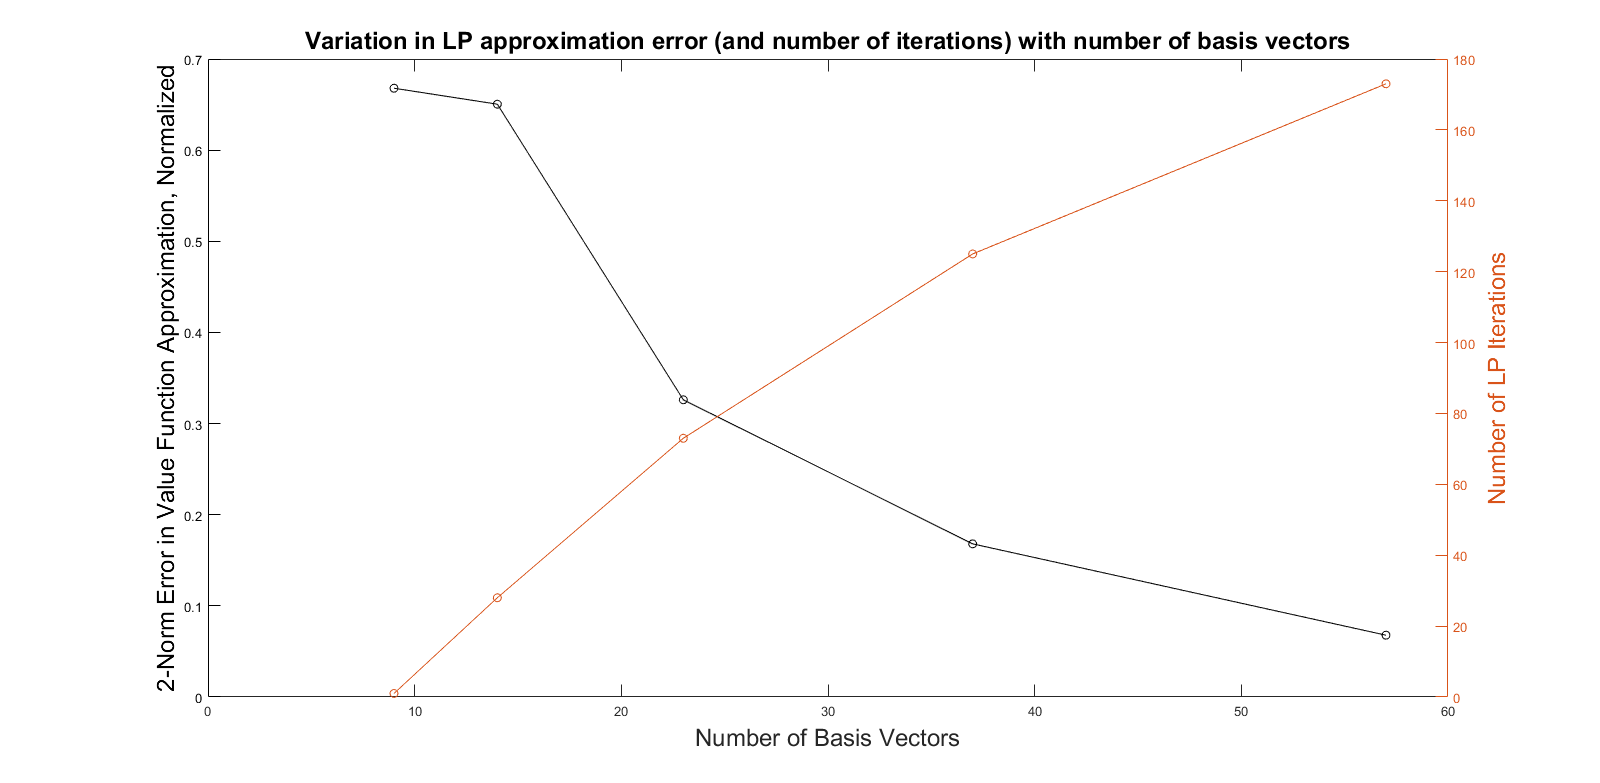
\includegraphics[scale=0.25]{ApproxErr_vs_NumIter.png}}
\caption{Variation in approximation error and solution time with number of basis functions added. Test size: $N_{1}=6$, $N_{2}=5$, $M=16$.}
\label{fig:ApproxVsIter}
\end{figure} This shows that the approximation error can indeed be made arbitarily small by adding more basis functions. %We may choose 



\section{Conclusion}
In conclusion, this paper has developed and optimized a model for energy transfers from two parallel storage devices to satisfy a random demand. The Markov decision process was formulated as a linear program, and approximated using monomials and state aggregations. The problem was then solved offline and tested online for the numerical example of an EV with hybrid energy storage. The final results confirm that the approximate LP does allow for determining an approximate optimal policy. Further work remains to be done to incorporate regenerative braking into this model.

\bibliographystyle{IEEEtran}
\bibliography{references.bib}

\end{document}